\documentclass[12pt]{report}
\usepackage[utf8]{inputenc}
\usepackage[bulgarian]{babel}
\usepackage{hyperref}
\setcounter{tocdepth}{4}
\setcounter{secnumdepth}{3}
\usepackage[backend=biber]{biblatex}
\usepackage{amsmath,amssymb}
\usepackage{systeme}
\usepackage[capitalise]{cleveref}
\usepackage{csquotes}
\usepackage[dvipsnames]{xcolor}
\usepackage{graphicx}
\usepackage{caption}
\usepackage{subcaption}
\usepackage{cancel}
\usepackage{breqn}
\usepackage{booktabs}
\usepackage{algorithm}
\usepackage[noend]{algpseudocode}
\usepackage{amsthm}
\usepackage{multicol}
\usepackage{listings}
\usepackage{amssymb}
\usepackage{pdfpages}
%\usepackage{subfigure}
\usepackage{multirow}
\usepackage{multicol}
\usepackage[toc,page]{appendix}\usepackage[abbreviations,symbols,style=index]{glossaries-extra}

\setquotestyle{english}

\newcommand{\norm}[1]{\left\lVert#1\right\rVert}
\newcommand{\dotprod}[2]{\left(#1, #2\right)}
\newcommand{\divg}[1]{\nabla\cdot#1}
\newcommand{\grad}[1]{\nabla#1}
\newcommand{\lapl}[1]{\Delta#1}
\newcommand{\vecf}[1]{\mathbf{#1}}

\addbibresource{main.bib}

\begin{document}
\begin{titlepage}
\begin{center}
\begin{minipage}{0.45\textwidth}
	
\includegraphics[scale=0.2]{Figures/2_SU_bg_n.png}
\end{minipage}
\begin{minipage}{0.45\textwidth}
	\footnotesize
	Софийски университет ``Св. Климент Охридски'' Факултет по математика и информатика\\
	\vfill
	Катедра ``Числени методи и алгоритми''
\end{minipage}

\vspace{1.5cm}

\textbf{\Large Имплементация на МКЕ за решаване на уравненията на Навие--Стокс за графични процесори}

\vspace{1.5cm}
\small
\textsc{Разширено резюме на дипломна работа}\\
\textsc{Магистърска програма ``Изчислителна математика и математическо моделиране''}
\vfill

\textbf{Дипломант:} Васил Д. Пашов, ФН 25938\\
\textbf{Научен ръководител:} гл. ас. д-р Тихомир Б. Иванов\\
\vfill
Ноември, 2021


\end{center}
\end{titlepage}

\begin{abstract}
В днешно време графичните процесори (GPU) са способни да извършват задачи с общо предназначение. Използването на графични процесори намира широко приложение за целите на криптовалутите, изкуствения интелект и т.н. Целта на тази дипломна работа е да се построи метод, базиран на МКЕ, за решаване на уравненията на Navier-Stokes. Методът е насочен за целите на компютърната графика, но може да бъде използван и в други областти.

Разглеждат се три различни подхода и се сравняват техните предимства и недостатъци спрямо поставените в дипломната работа цели -- добра производителност и възможност за ефективна имплементация за графични процесори. Проведени са числени експерименти, базирани на класическата моделна задача -- 2D DFG Benchmark. Алгоритъмът, който най-добре изпънява поставените цели, разделя оператора по времето на три части, всяка от които е имплементирана по метод така, че да се възползва се от графичния процесор.
\end{abstract}

\tableofcontents
\chapter{Въведение}
През последните 20 години графичните процесори (GPU) изминаха дълъг път от фиксирана програмна рамка, използвана само за целите на компютърната графика, до това да станат напълно способни да изпълняват задачи с общо предназначение. Тази еволюция направи възможно използването на изчислителната мощност на графичните процесори в области, различни от компютърната графика, като изкуствен интелект, криптовалути, флуидна динамика и т.н.

Въпреки че графичните процесори имат повече ядра от централния процесор (CPU), сравнението между двете, базирано само на броя на ядрата, не е подходящо поради огромната разлика в хардуерната архитектура. Не всеки алгоритъм може да бъде ефективно реализиран за изпълнение върху GPU. Отново поради разликата в архитектурата, даден алгоритъм няма да се възползва напълно от изчислителната мощност на графичния процесор просто чрез пренаписването му в специфичен за графичния процесор език. При изчислителния модел на GPU, нишките, които изпълняват конкретна задача, изпълняват (едновременно) една и съща инструкция, но върху различен набор от данни. Това прави графичния процесор идеален за проблеми, които имат висока аритметична интензивност с ниски зависимости между данните.

\section{GPU реализация за МКЕ}
Можем да разбием компютърната имплементация на МКЕ на три подзадачи. Първо, областта трябва да бъде дискретизирана. Това е задачата, в която графичният процесор е най-малко полезен поради естеството на проблема. Задачата е частично разгледана в \cite{meshing}. Второ, поелементните изчисления и асемблирането на глобалните матрици са разгледани в \cite{assembling}. Като се има предвид, че поелементните изчисления са независими едно от друго, можем да получим значително забързване чрез GPU реализация, но това е така, само ако матриците не се съхраняват в разреден формат. Повечето от разредените матрични формати създават зависимости между данните, което прави по-трудна задачата за паралелно асемблиране на глобалните матрици. Трето, в резултат от прилагането на МКЕ получаваме една или повече линейни (или нелинейни) системи, които трябва да бъдат решени. В общия случай решаването им е най-времеемката стъпка. За големи системи линейни уравнения се предпочитат итеративни методи, като най-често се използват методът на спрегнатия градиент (и негови прозиводни) и GMRES. Решаването на линейни системи е разгледано в \cite{sparse-solvers}, \cite{matrix-vector-mult}, \cite{biconjugate}.

\section{Цели и структура на дипломната работа}

Основните цели на дипломната работа са:
\begin{itemize}
    \item Построяване на метод, базиран на МКЕ, за решаване на уравненията на Navier-Stokes за несвиваеми Нютонови флуиди. Методът е предназначен за целите на комютърната графика, но може да бъде използван и в други области. За целите на компютърната графика поставяме следните изисквания:
    \begin{itemize}
        \item Бързодействие на метода;
        \item Възможност за ефективна паралелизация на множество (CPU) ядра;
        \item Възможност за ефективна GPU имплементация, т.е. методът трябва да има висока артиметична итензивност, но слаби зависимости между данните;
        \item Възможност за работа с произволна по големина стъпка по времето, без от нея да зависи дискретизацията на областта. Това често се налага в компютърната графика, тъй като видео клиповете най-често имат 24, 30 или 60 кадъра в секунда, а останалите кадри се игнорират;
    \end{itemize}
    \item Провеждане на числени експерименти с цел установяване ефективността на избрания метод. Експериментите са базирани на класическата моделна задача -- 2D DFG Benchmark;
    \item Да се коментират плюсовете и минусите на GPU имплементацията;
    \item Да се дадат предложения за бъдещо развитие на алогоритъма.
\end{itemize}


Дипломната работа е структурирана, както следва. Гл. \ref{ch:FEM-NS} представя диференциалната постановка на задачата и сравнява три различни подхода за решаването \'{и}. Два от методите използват разделяне на диференциалния оператор по времето, а третият подход е директен. Представени са още формат за съхраняване на разредени матрици, методът на спрегнатия градиент и метод за преобуславяне. Гл. \ref{ch:FEM-Parallel} представя детайли относно паралелната (CPU) имплементация, както и GPU имплементацията на един от алгоритмите, представени в Гл. \ref{ch:FEM-NS}. Представени са резултати за това как производителността на избраните алгоритми се скалира с добавяне на (логически CPU) ядра, направено е сравнение между CPU и GPU имплементациите. 

\section{Компютърен код}
Компютърната имплементация на алгоритъма, описан в тази дипломна работа, може да бъде намерен в GitHub.
\begin{itemize}
    \item За целите на работата беше разработена библиотека за работа с разредени матрици, имплементирана в C++. В нея са включени класове за работа с разредени матрици в CSR формат както и паралелни имплементации на метода на спрегнатия градиент (както и някои негови вариации). Библиотеката може да бъде намерена на следната страница: \url{https://github.com/vasil-pashov/sparse_matrix_math}
    \item Кодът, имплементиращ метода на крайните елементи, може да бъде намерен на следната страница: \url{https://github.com/vasil-pashov/Navier_Stokes_FEM}
\end{itemize}

\chapter{МКЕ за уравненията на Navier-Stokes}\label{ch:FEM-NS}
\section{Уравнения на  Navier-Stokes}
Нека формулираме уравненията, както са представени в \cite{Larson-Bengzon}.
\begin{equation}
\begin{aligned}
  % Conservation of momentum
  \frac{\partial \mathbf{u}(\mathbf{x}, t)}{\partial t} + \left(\mathbf{u}(\mathbf{x}, t)\cdot\nabla\right)\mathbf{u}(\mathbf{x}, t) + \nabla p(\mathbf{x}, t) - \nu\Delta\mathbf{u}(\mathbf{x}, t) &= \mathbf{f}(\mathbf{x}, t)\\
  % Continuity
  \nabla \cdot \mathbf{u}(\mathbf{x}, t) &= 0
\end{aligned}\label{eq:NS}
\end{equation}

където:
\begin{itemize}
  \item $\mathbf{u} \in \mathbb{R}^n$ е скоростта;
  \item $p \in \mathbb{R}$ е налягането;
  \item $\nu$ е вискозитет;
  \item $\mathbf{f}$ е съвкупност от обемни сили, напр. гравитация.
\end{itemize}
\section{Моделна задача}
Разглеждаме постановката 2D DFG Benchmark \cite{dfg-problem}. Задачата разглежда поток в канал с препятствие. Каналът е правоъгълник с дължина $2.2$ и височина $0.41$. Препятствието е окръжност с център $(0.2, 0.2)$ и диаметър $0.1$ (вж. Фиг. \ref{fig:2D_DFG_Benchmark}). Граничните условия са, както следва:

\begin{align*}
  &\mathbf{u} = 0, &&\left(\mathbf{x}, t\right) \in \left(\Gamma_1 \cup \Gamma_3 \cup \Gamma_5\right) \times J \\
  &\mathbf{u} = \mathbf{u}_{\Gamma_4}, &&\left(\mathbf{x}, t\right) \in \Gamma_4 \times J \\
  &\nu\frac{\partial\mathbf{u}}{\partial\mathbf{n}} - p\mathbf{n} = 0, &&\left(\mathbf{x}, t\right) \in \Gamma_2 \times J
\end{align*}
където за ламинарен поток $\mathbf{u}_{\Gamma_4}=\left(\frac{1.2y\left(0.41 - y\right)}{0.41^2}, 0\right)$, а за турбулентен $\mathbf{u}_{\Gamma_4}=\left(\frac{6y(0.41-y)}{0.41^2}, 0\right)$,

\begin{figure}[H]
  \centering
  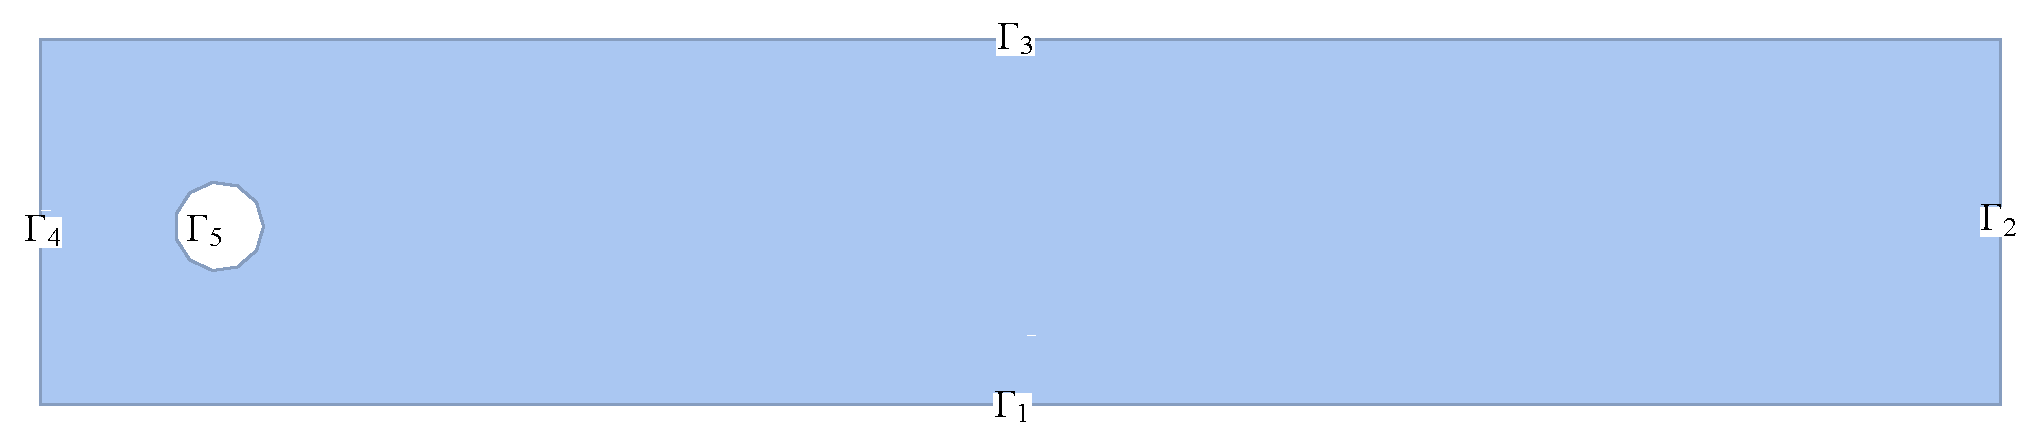
\includegraphics[scale=0.39]{Figures/02_model_problem/2D_DFG_Benchmark.pdf}
  \caption{Геометрия на моделната задача 2D DFG Benchmark}
  \label{fig:2D_DFG_Benchmark}
\end{figure}

\section{Метод на крайните елементи}
\subsection{Директен подход}
Един възможен подход за числено решаване на уравненията на Navier-Stokes е да разгледаме слабата формулировка на (\ref{eq:NS}) и да приложим МКЕ върху нея. Според \cite{gresho-fem} при този подход са подходящи само неявни схеми за дискретизация по времето. Основният недостатък на този подход е, че на всяка стъпка по времето трябва да бъде решена една нелинейна система. За дискретизацията по времето е използван метод на Кранк-Никълсън. Представяме финалната постановка на метода (вж. (\ref{eq:2D_DFG_Direct_Crank-Nicholson})), която е подробно изведена в дипломната работа. Да се намерят $\mathbf{u}_h = \sum\limits_{i=1}^{2N_v}{\mathbf{\Phi}_iq_i} \in U_h \subset U : \left\{\mathbf{v} \in H^1 : \mathbf{v}(\mathbf{x}, t)|_{\Gamma_1 \cup \Gamma_3 \cup \Gamma_5} = 0\right\}$  и $p_h = \sum\limits_{i=1}^{N_p}{\chi_ip_i} \in Q_h \subset L^2$, където $N_v$ е броят на възлите за скоростта, които не лежат върху $\Gamma_1 \cup \Gamma_3 \cup \Gamma_5$, а $N_p$ е броят на възлите за налягането, $  \{\mathbf{\Phi}_i\}^{2N_v}_{i=1} = \left\{
  \begin{bmatrix} \phi_1 \\ 0\end{bmatrix}
  , \dots ,
  \begin{bmatrix} \phi_{N_v} \\ 0\end{bmatrix}
  ,
  \begin{bmatrix} 0 \\ \phi_1\end{bmatrix}
  , \dots ,
  \begin{bmatrix} 0 \\ \phi_{N_v}\end{bmatrix}
  \right\}$ са базисните функции за пространството $U_h$, а $\left\{\chi_i\right\}^{N_p}_{i = 1}$ са базисните функции за пространството $Q_h$.
\begin{multline}\label{eq:2D_DFG_Direct_Crank-Nicholson}
	\begin{bmatrix}
		\mathbf{M}+\frac{\Delta t}{2}\left(\nu\mathbf{K}+\mathbf{C}(\mathbf{u}_h^{i+1})\right) & 0 & -\frac{\Delta t}{2}\mathbf{B}^T_1 \\
		0 &\mathbf{M}+\frac{\Delta t}{2}\left(\nu\mathbf{K}+\mathbf{C}(\mathbf{u}_h^{i+1})\right) & -\frac{\Delta t}{2}\mathbf{B}^T_2 \\
		-\frac{\Delta t}{2}\mathbf{B}_1 & -\frac{\Delta t}{2}\mathbf{B}_2 & 0
	\end{bmatrix}
	\begin{bmatrix}
		\mathbf{Q}_1^{i+1}\\
		\mathbf{Q}_2^{i+1}\\
		\mathbf{P}^{i+1}
	\end{bmatrix} = \\
	\begin{bmatrix}
		\mathbf{M}-\frac{\Delta t}{2}\left(\nu\mathbf{K}+\mathbf{C}(\mathbf{u}_h^{i})\right) & 0 & \frac{\Delta t}{2}\mathbf{B}^T_1 \\
		0 &\mathbf{M}-\frac{\Delta t}{2}\left(\nu\mathbf{K}+\mathbf{C}(\mathbf{u}_h^{i})\right) & \frac{\Delta t}{2}\mathbf{B}^T_2 \\
		\frac{\Delta t}{2}\mathbf{B}_1 & \frac{\Delta t}{2}\mathbf{B}_2 & 0
	\end{bmatrix}
	\begin{bmatrix}
		\mathbf{Q}_1^{i}\\
		\mathbf{Q}_2^{i}\\
		\mathbf{P}^{i}
	\end{bmatrix}
\end{multline}
Където $\mathbf{M}$ е матрицата на масата
\begin{equation*}
	\mathbf{M} =
	\begin{bmatrix}
		\left(\phi_1, \phi_1\right) & \left(\phi_2, \phi_1\right) & \cdots & \left(\phi_{N_v}, \phi_1\right) \\
		\left(\phi_1, \phi_2\right) & \left(\phi_2, \phi_2\right) & \cdots & \left(\phi_{N_v}, \phi_2\right) \\
		\vdots & \vdots & \cdots & \vdots \\
		\left(\phi_1, \phi_{N_v}\right) & \left(\phi_2, \phi_{N_v}\right) & \cdots & \left(\phi_{N_v}, \phi_{N_v}\right)
	\end{bmatrix}
\end{equation*}
$\mathbf{C}$ е конвективната матрица
\begin{equation*}
	\mathbf{C}(\mathbf{u}_h) = \begin{bmatrix}
		\left(\mathbf{u}_h\cdot\nabla\phi_1, \phi_1\right) & \left(\mathbf{u}_h\cdot\nabla\phi_2, \phi_1\right) & \cdots & \left(\mathbf{u}_h\cdot\nabla\phi_{N_v}, \phi_1\right)\\
		\left(\mathbf{u}_h\cdot\nabla\phi_1, \phi_2\right) & \left(\mathbf{u}_h\cdot\nabla\phi_2, \phi_2\right) & \cdots & \left(\mathbf{u}_h\cdot\nabla\phi_{N_v}, \phi_2\right)\\
		\vdots & \vdots & \cdots & \vdots \\
		\left(\mathbf{u}_h\cdot\nabla\phi_1, \phi_{N_v}\right) & \left(\mathbf{u}_h\cdot\nabla\phi_2, \phi_{N_v}\right) & \cdots & \left(\mathbf{u}_h\cdot\nabla\phi_{N_v}, \phi_{N_v}\right)
	\end{bmatrix}
\end{equation*}
$\mathbf{K}$ е матрица на коравина
\begin{equation*}
	\mathbf{K} = \begin{bmatrix}
		\left(\nabla\phi_1\cdot\nabla\phi_1\right) & \left(\nabla\phi_2\cdot\nabla\phi_1\right) &
		\cdots &
		\left(\nabla\phi_{N_v}\cdot\nabla\phi_1\right) \\
		\left(\nabla\phi_1\cdot\nabla\phi_2\right) & \left(\nabla\phi_2\cdot\nabla\phi_2\right) &
		\cdots &
		\left(\nabla\phi_{N_v}\cdot\nabla\phi_2\right) \\
		\vdots & \vdots & \cdots & \vdots \\
		\left(\nabla\phi_1\cdot\nabla\phi_{N_v}\right) & \left(\nabla\phi_2\cdot\nabla\phi_{N_v}\right) &
		\cdots &
		\left(\nabla\phi_{N_v}\cdot\nabla\phi_{N_v}\right)
	\end{bmatrix}
\end{equation*}

\begin{equation*}
	\mathbf{B}_1 = \begin{bmatrix}
		\left(\frac{\partial\phi_1}{\partial x_1}, \chi_1\right) & \left(\frac{\partial\phi_2}{\partial x_1}, \chi_1\right) & \cdots & \left(\frac{\partial\phi_{N_v}}{\partial x_1}, \chi_1\right) \\
		\left(\frac{\partial\phi_1}{\partial x_1}, \chi_2\right) & \left(\frac{\partial\phi_2}{\partial x_1}, \chi_2\right) & \cdots & \left(\frac{\partial\phi_{N_v}}{\partial x_1}, \chi_2\right) \\
		\vdots & \vdots & \cdots & \vdots \\
		\left(\frac{\partial\phi_1}{\partial x_1}, \chi_{N_p}\right) & \left(\frac{\partial\phi_2}{\partial x_1}, \chi_{N_p}\right) & \cdots & \left(\frac{\partial\phi_{N_v}}{\partial x_1}, \chi_{N_p}\right)
	\end{bmatrix}
\end{equation*}

\begin{equation*}
\mathbf{B}_2 = \begin{bmatrix}
\left(\frac{\partial\phi_1}{\partial x_2}, \chi_1\right) & \left(\frac{\partial\phi_2}{\partial x_2}, \chi_1\right) & \cdots & \left(\frac{\partial\phi_{N_v}}{\partial x_2}, \chi_1\right) \\
\left(\frac{\partial\phi_1}{\partial x_2}, \chi_2\right) & \left(\frac{\partial\phi_2}{\partial x_2}, \chi_2\right) & \cdots & \left(\frac{\partial\phi_{N_v}}{\partial x_2}, \chi_2\right) \\
\vdots & \vdots & \cdots & \vdots \\
\left(\frac{\partial\phi_1}{\partial x_2}, \chi_{N_p}\right) & \left(\frac{\partial\phi_2}{\partial x_2}, \chi_{N_p}\right) & \cdots & \left(\frac{\partial\phi_{N_v}}{\partial x_2}, \chi_{N_p}\right)
\end{bmatrix}
\end{equation*}

\subsection{Разделяне на диференциалния оператор по времето}
Както беше споменато, според \cite{gresho-fem}, за директния подход са приложими само неявни схеми за дискретизация по времето. Такива схеми обаче изискват решаване на нелинейни системи, както и асемблиране на матрицата $C(\mathbf{u}_h)$ на всяка стъпка по времето. Това прави методите бавни и неудобни за паралелна имплементация. Друг възможен подход е операторът по времето да бъде разделен. Двете разделяния, които ще представим, са описани в \cite{Bridson} и \cite{Chorin-operator-split}. За дискретизацията по времето е използвана явна схема. И двата подхода изискват да бъде решено уравнение на Поасон относно налягането. Това налага полиномиалното пространство на елементите относно налягането да бъде поне от първи ред.
\subsubsection{Разделяне на Chorin}
При това разделяне диференцианият оператор по времето се разделя на две части. Една част, отговаряща за адвекцията и дифузията, и една част, отговаряща за налягането. МКЕ има следния вид (за подробно извеждане вж. дипломната работа).
\begin{equation}
\begin{aligned}
	\begin{bmatrix}
		\mathbf{M} & 0 \\
		0 & \mathbf{M}
	\end{bmatrix}
	\begin{bmatrix}
		\vecf{Q^{i + \frac{1}{2}}_1} \\
		\vecf{Q^{i + \frac{1}{2}}_2}
	\end{bmatrix} &=
	\begin{bmatrix}
		\mathbf{M} & 0 \\
		0 & \mathbf{M}
	\end{bmatrix}
	\begin{bmatrix}
		\vecf{Q^{i}_1} \\
		\vecf{Q^{i}_2}
	\end{bmatrix} - \Delta t \begin{bmatrix}
		\nu \mathbf{K} + \mathbf{C}(\vecf{u_h}) & 0 \\
		0 & \nu \mathbf{K} + \mathbf{C}(\vecf{u_h})
	\end{bmatrix} \begin{bmatrix}
		\vecf{Q^i_1} \\
		\vecf{Q^i_2}
	\end{bmatrix} \\
	\mathbf{K_p}\vecf{P}^i &= -\frac{1}{\Delta t} \begin{bmatrix}
		\mathbf{B_1} & \mathbf{B_2}
	\end{bmatrix} \begin{bmatrix}
		\vecf{Q^{i + \frac{1}{2}}_1} \\
		\vecf{Q^{i + \frac{1}{2}}_2}
	\end{bmatrix} \\
	\begin{bmatrix}
		\mathbf{M} & 0 \\
		0 & \mathbf{M}
	\end{bmatrix} \begin{bmatrix}
		\vecf{Q^{i+1}_1} \\
		\vecf{Q^{i+1}_2}
	\end{bmatrix} &=	\begin{bmatrix}
		\mathbf{M} & 0 \\
		0 & \mathbf{M}
	\end{bmatrix} \begin{bmatrix}
		\vecf{Q^{i+\frac{1}{2}}_1} \\
		\vecf{Q^{i+\frac{1}{2}}_2}
	\end{bmatrix} - \Delta t \begin{bmatrix}
		\vecf{B_{p,1}} \\
		\vecf{B_{p,2}}
	\end{bmatrix} \vecf{P}^i
\end{aligned}\label{eq:chorin_split_fem}
\end{equation}

\begin{equation*}
	\mathbf{K_p} = \begin{bmatrix}
		\dotprod{\grad{\chi_1}}{\grad{\chi_1}} & \dotprod{\grad{\chi_2}}{\grad{\chi_1}} & \dots & \dotprod{\grad{\chi_{Np}}}{\grad{\chi_1}}\\
		\dotprod{\grad{\chi_1}}{\grad{\chi_2}} & \dotprod{\grad{\chi_2}}{\grad{\chi_2}} & \dots & \dotprod{\grad{\chi_{Np}}}{\grad{\chi_2}}\\
		\vdots & \vdots & \vdots & \vdots\\
		\dotprod{\grad{\chi_1}}{\grad{\chi_{Np}}} & \dotprod{\grad{\chi_2}}{\grad{\chi_{Np}}} & \dots & \dotprod{\grad{\chi_{Np}}}{\grad{\chi_{Np}}}
	\end{bmatrix}
\end{equation*}
\begin{equation*}
	\mathbf{B_{p,1}} = \begin{bmatrix}
		\left(\frac{\partial\chi_1}{\partial x_1}, \phi_1\right) & \left(\frac{\partial\chi_2}{\partial x_1}, \phi_1\right) & \cdots & \left(\frac{\partial\chi_{N_p}}{\partial x_1}, \phi_1\right) \\
		\left(\frac{\partial\chi_1}{\partial x_1}, \phi_2\right) & \left(\frac{\partial\chi_2}{\partial x_1}, \phi_2\right) & \cdots & \left(\frac{\partial\chi_{N_p}}{\partial x_1}, \phi_2\right) \\
		\vdots & \vdots & \cdots & \vdots \\
		\left(\frac{\partial\chi_1}{\partial x_1}, \phi_{N_v}\right) & \left(\frac{\partial\chi_2}{\partial x_1}, \phi_{N_v}\right) & \cdots & \left(\frac{\partial\chi_{N_v}}{\partial x_1}, \phi_{N_v}\right)
	\end{bmatrix}
\end{equation*}
\begin{equation*}
	\mathbf{B_{p,2}} = \begin{bmatrix}
		\left(\frac{\partial\chi_1}{\partial x_2}, \phi_1\right) & \left(\frac{\partial\chi_2}{\partial x_2}, \phi_1\right) & \cdots & \left(\frac{\partial\chi_{N_p}}{\partial x_2}, \phi_1\right) \\
		\left(\frac{\partial\chi_1}{\partial x_2}, \phi_2\right) & \left(\frac{\partial\chi_2}{\partial x_2}, \phi_2\right) & \cdots & \left(\frac{\partial\chi_{N_p}}{\partial x_2}, \phi_2\right) \\
		\vdots & \vdots & \cdots & \vdots \\
		\left(\frac{\partial\chi_1}{\partial x_2}, \phi_{N_v}\right) & \left(\frac{\partial\chi_2}{\partial x_2}, \phi_{N_v}\right) & \cdots & \left(\frac{\partial\chi_{N_v}}{\partial x_2}, \phi_{N_v}\right)
	\end{bmatrix}
\end{equation*}

\subsection{Разделяне на адвекцията и дифузията}
Разделянето на Chroin може да бъде комбинирано с явни схеми за диференциране по времето, но има няколко недостатъка. От една страна, комбинацията от дифизуя и адвекция в едно уравнение обвързва стъпката по времето и размера на елементите. При работа с фиксиран брой кадри (фиксирана стъпка) в секунда, за да имаме устойчивост, трябва или да използваме по-фина мрежа, или да намалим стъпката по времето и да използваме само някои кадри, което е загуба на изчислителен ресурс и време. Един възможен подход е да използваме неявна схема за апроксимиране на дифузията и адвекцията. Това отново би наложило решаване на нелинейна система, както и асемблиране на матрицата $C(\mathbf{u}_h)$ на всяка стъпка по времето. Полунеявна схема би могла да бъде решение на този проблем, ние обаче ще разделим уравнението за дифузия-адвекция още веднъж. Ползите от това са две: първо, за адвекцията съществува устойчив (независимо от големината на стъпката по времето) алгоритъм \cite{semi-lagrangian-stability}, който е изключително удобен за паралелна имплементация, както на CPU, така и на GPU. Второ, за дифузията можем да приложим неявна схема, без да се налага решаване на нелинейна система. МКЕ има следния вид (вж. (\ref{eq:adv-diff-split-advect})-(\ref{eq:adv-diff-split-velicity-mass}), където (\ref{eq:adv-diff-split-advect}) е полу-Лагранжевият метод).

\begin{align}
	&\mathbf{Q^A} = advect(KDTree, \mathbf{Q^{i}}, \Delta t) \label{eq:adv-diff-split-advect}\\
		&\left(\begin{bmatrix}
		\mathbf{M} & 0 \\
		0 & \mathbf{M}
	\end{bmatrix} + \nu\Delta t\begin{bmatrix}
		\mathbf{K} & 0 \\
		0 & \mathbf{K}
	\end{bmatrix}\right)\begin{bmatrix}
		\vecf{Q^{B}_1} \\
		\vecf{Q^{B}_2}
	\end{bmatrix} = \begin{bmatrix}
		\mathbf{M} & 0 \\
		0 & \mathbf{M}
	\end{bmatrix}\begin{bmatrix}
		\vecf{Q^{A}_1} \\
		\vecf{Q^{A}_2}
	\end{bmatrix} \label{eq:adv-diff-split-diffuse}\\
	&\mathbf{K_p}\vecf{P}^i = -\frac{1}{\Delta t} \begin{bmatrix}
		\mathbf{B_1} & \mathbf{B_2}
	\end{bmatrix} \begin{bmatrix}
		\vecf{Q^{B}_1} \\
		\vecf{Q^{B}_2}
	\end{bmatrix} \label{eq:adv-diff-split-pressure}\\
	&\begin{bmatrix}
		\mathbf{M} & 0 \\
		0 & \mathbf{M}
	\end{bmatrix} \begin{bmatrix}
		\vecf{Q^{i+1}_1} \\
		\vecf{Q^{i+1}_2}
	\end{bmatrix} =	\begin{bmatrix}
		\mathbf{M} & 0 \\
		0 & \mathbf{M}
	\end{bmatrix} \begin{bmatrix}
		\vecf{Q^{B}_1} \\
		\vecf{Q^{B}_2}
	\end{bmatrix} - \Delta t \begin{bmatrix}
		\vecf{B_{p,1}} \\
		\vecf{B_{p,2}}
	\end{bmatrix} \vecf{P}^i \label{eq:adv-diff-split-velicity-mass}
\end{align}
\subsubsection{Полу-Лагранжев метод за пресмятане на адвекция}
Полу-Лагранжевият метод се базира на факта, че решаването на $\frac{\partial\vecf{u}}{\partial t} + \vecf{u}\cdot\grad{u} = 0$ е тривиално, ако разгледаме задачата в Лагранжева постановка. Нека си представим, че можем да проследим всяка една частица от флуида. Тогава, за да намерим скоростта на флуида в дадена точка, трябва само да намерим коя частица се намира в нея и да вземем нейната скорост. Работата директно с частици обаче има своите недостатъци \cite{Bridson}. За да се справим с тях, ще използваме комбинация между Ойлерова и Лагранжева постановка на задачата. За да намерим скоростта в точка $\mathbf{x_e}$ в момент от време $t + \Delta t$ е нужно да намерим частицата с позиция $\mathbf{x_s}$ (в момент $t$), която ще се премести в точка $\mathbf{x_e}$ в момент $t + \Delta t$. За тази цел ще линеализираме задачата, като разглеждаме полето на скоростите в точката $\mathbf{x_e}$ в момент от време $t$ и се придвижваме със стъпка $\Delta t$ ``назад'' в полето на скоростта. Това ни дава приблизителната позиция $\mathbf{x_s}$ на частицата, която би се озовала в точка $\mathbf{x_e}$ след период от време $\Delta t$. Тази позиция $\mathbf{x_s}$ обаче най-вероятно няма да бъде възел от триангулацията, по тази причина трябва да интерполираме между стойностите на възлите в елемента. Очевидно е, че пресмятането на една скорост не зависи от другите скорости, които се пресмятат в момента. Това прави алгоритъма изключително подходящ за паралелна имплементация както на CPU, така и на GPU.       
\subsection{Избор на крайни елементи}
За уравнение (\ref{eq:2D_DFG_Direct_Crank-Nicholson}) използваме неконформния елемент на Crouzeix-Raviart (вж. Фиг. \ref{fig:P1P0-CR-Standard}). Предимствата му са, че поддържа нулева дивергенция и че е евтин от изчислителна гледна точка. Използването на този елемент би генерирало по-малка система, в сравнение с елемент, чиито полиномиални пространства за скоростта и налягането са от по-висок ред. За подходите, използващи разделяне на оператора по времето, използваме елемент на Taylor-Hood (вж. Фиг. \ref{fig:P2P1-Standard}). Според \cite{gresho-fem} това е ``най-простият елемент от втори ред'' и ``първоначален фаворит''.

\begin{figure}[H]
  \centering
  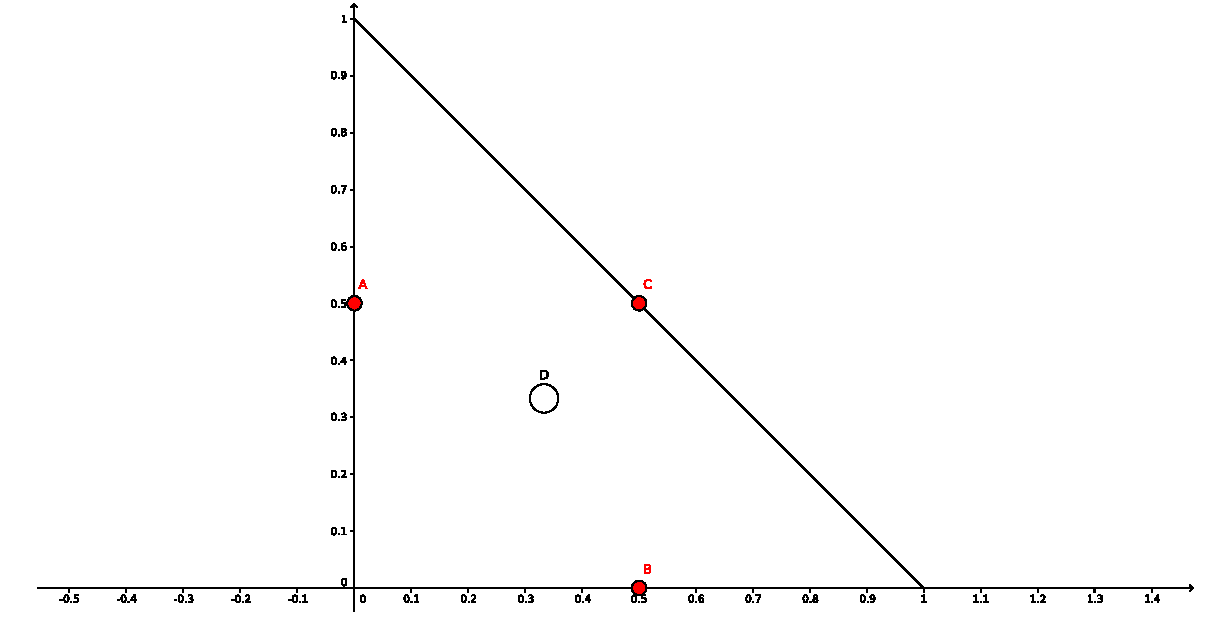
\includegraphics[width=\textwidth]{Figures/01_introduction/cr_element.pdf}
  \caption{Неконформен елемент на Crouzeix-Raviart. Трите степени на свобода за скоростта са отбелязани със запълнен кръг, степента на свобода за налягането е отбелязана с окръжност.}\label{fig:P1P0-CR-Standard}
\end{figure}

\begin{figure}[H]
  \centering
  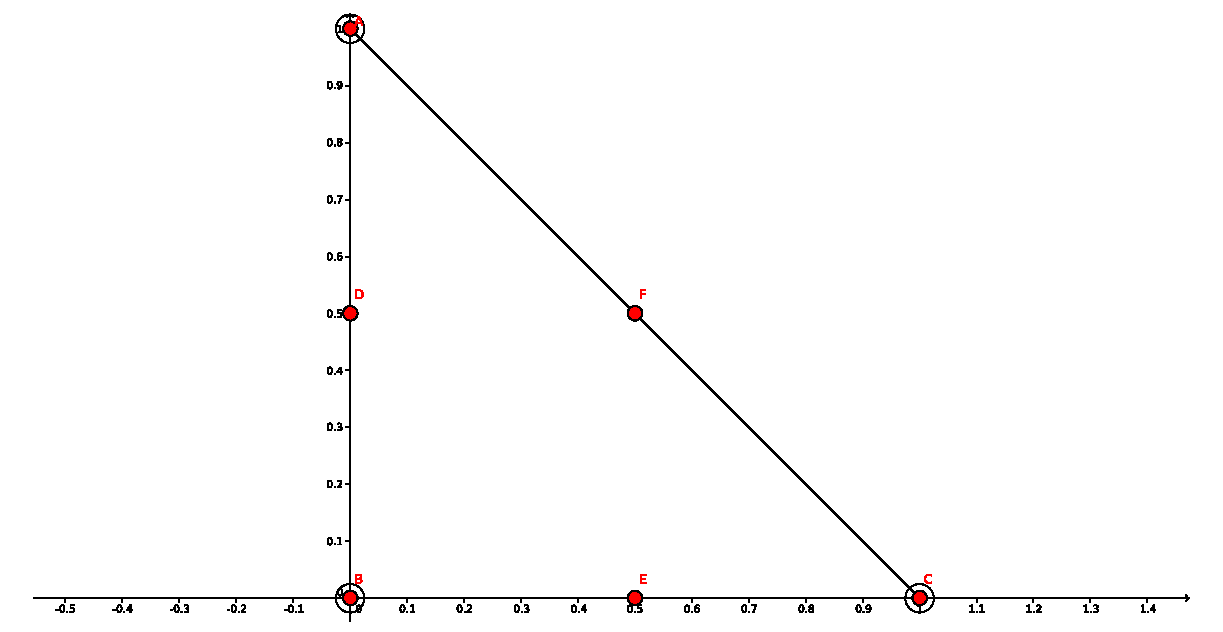
\includegraphics[width=\textwidth]{Figures/01_introduction/tylor_hood_element.pdf}
  \caption{Елемент на Taylor-Hood от втори ред. Шестте степени на свобода за скоростта са отбелязани със запълнен кръг, трите степени на свобода за налягането са отбелязани с окръжност.}\label{fig:P2P1-Standard}
\end{figure}

\section{CSR формат за съхранение на разредени матрици}
Нека бележим броя на ненулеви елементи в дадена матрица с $nnz$, а броя на редовете -- с $m$. За представянето ѝ в CSR формат са нужни три масива: $NZ$ с размер $nnz$, в който са записани ненулевите елементи на матрицата, $Pos$ с размер $nnz$, в който е записан индексът на стълба на всеки един елемент от $NZ$ и $Start$ с размер $m+1$, в който е записан индексът в $NZ$ (и $Pos$) където започва $i$-тият ред, последният елемент има стойност $nnz$. Изискване е редовете да са подредени във възходящ ред в паметта. Следва илюстрация (вж. Фиг. \ref{fig:example_csr_sparse_matrix}) на формата, приложен за матрицата от Фиг. \ref{fig:example_sparse_matrix}
\begin{figure}[H]
$$
\begin{bmatrix}
	1 & 0 & 0 & 2 & 0\\
	0 & 0 & 3 & 4 & 0\\
	0 & 0 & 5 & 0 & 6\\
	0 & 0 & 0 & 0 & 0\\
	7 & 0 & 8 & 9 & 0
\end{bmatrix}
$$
\caption{Примерна разредена матрица}\label{fig:example_sparse_matrix}
\end{figure}

\begin{figure}[H]
\centering
\begin{tabular}{l|ccccccccc}
\cline{2-10}
\textit{NZ}    & 1 & 2 & 3 & 4 & 5 & 6                      & 7 & 8 & \multicolumn{1}{c|}{9} \\ \cline{2-10}
\textit{Pos}   & 0 & 3 & 2 & 3 & 2 & 4                      & 0 & 2 & \multicolumn{1}{c|}{3} \\ \cline{2-10}
\textit{Start} & 0 & 2 & 4 & 6 & 6 & \multicolumn{1}{c|}{9} &   &   &                        \\ \cline{2-7}
\end{tabular}\caption{Матрицата от Фиг. \ref{fig:example_sparse_matrix} в CSR формат. Индексацията на масивите започва от 0.}\label{fig:example_csr_sparse_matrix}
\end{figure}

\section{Метод на спрегнатия градиент}
Всички ленейни алгебрични системи, участващи в получената по МКЕ дискретна задача имат симетрични и положително определени матрици. Един от най-популярните методи за решаване на такива системи е методът на спрегнатия градиент. Подробна информация за него може да се намери в \cite{saad-sparse}. Тук ще приложим псевдокод за алгоритъма (вж. Алг. \ref{alg:CG})

\begin{algorithm}[H]
\centering
\floatname{algorithm}{Алгоритъм}
\caption{Метод на спрегнатия градиент за решаване на $Ax=b$ с начално приближение $x_0$}\label{alg:CG}
\begin{algorithmic}[]
		\Procedure{CG}{$A, b, x_0$}
			\State $r_0 \gets b - Ax_0$
			\State $p_0 \gets r_0$
			\For{$j \gets 0, 1, \dots$ until convergence}
				\State $\alpha_j \gets \frac{(r_j, r_j)}{(Ap_j, p_j)}$
				\State $x_{j+1} \gets x_j + \alpha_j p_j$
				\State $r_{j+1} \gets r_j - \alpha_j Ap_j$
				\State $\beta_j \gets \frac{(r_{j+1}, r_{j+1})}{(r_j, r_j)}$
				\State $p_{j+1} \gets r_{j+1} + \beta_j p_j$
			\EndFor
			\State \Return $x_{j+1}$
		\EndProcedure
\end{algorithmic}
\end{algorithm}

\section{Непълна факторизация по Холецки с нулево запълване (IC0)}
Разглеждаме линейната система $Ax=b$. Често използвана техника при итеративните методи е преобуславянето. Целта е да бъде подобрено числото на обусловеност на матрицата. За тази цел двете страни на системата се умножават с матрица $P^{-1} \approx A^{-1}$. Добре е след преобуславяне, матрицата да запазва най-важните си свойства (да продължава да бъде симетрична и/или положително определена). В общия случай, дори и $A$ и $P^{-1}$ да бъдат разредени матрици, тяхното произведение няма да бъде разредена матрица. По тази причина е желателно да не умножаваме матрицата $A$ по преобуславящата матрица. Представяме един възможен алгоритъм (вж. Алг. \ref{alg:pcg}), при който не се налага такова умножение. За повече информация вж. \cite{saad-sparse}.

\begin{algorithm}[H]
\centering
\floatname{algorithm}{Алгоритъм}
\caption{Преобусловен метод на спрегнатия градиент за решаване на $Ax=b$ с начално приближение $x_0$}\label{alg:pcg}
\begin{algorithmic}[1]
		\Procedure{PCG}{$A, M^{-1} b, x_0$}
			\State $r_0 \gets b - Ax_0$
			\State $z_0 \gets M^{-1}r_0$\label{alg-line:apply-preconditioner}
			\State $p_0 \gets z_0$
			\For{$j \gets 0, 1, \dots$ until convergence}
				\State $\alpha_j \gets \frac{(r_j, z_j)}{(Ap_j, p_j)}$
				\State $x_{j+1} \gets x_j + \alpha_j p_j$
				\State $r_{j+1} \gets r_j - \alpha_j Ap_j$
				\State $z_{j+1} \gets M^{-1}r_{j+1}$
				\State $\beta_j \gets \frac{(r_{j+1}, z_{j+1})}{(r_j, z_j)}$
				\State $p_{j+1} \gets z_{j+1} + \beta_j p_j$
			\EndFor
			\State \Return $x_{j+1}$
		\EndProcedure
\end{algorithmic}
\end{algorithm}

При симетрични и положително определени матрици е логично да използваме факторизация на Холецки $A=LL^T$ за преобуславяне. В общия случай, дори $A$ да бъде разредена матрица, матрицата $L$ не е разредена. По тази причина търсим матрица $\tilde{L} \approx L$, такава че $\tilde{L}\tilde{L^T} \approx A$. Ще поискаме $\tilde{L}$ да има ненулеви елементи само там където долнотриъгълната част от $A$ има ненулеви елементи. Тези ненулеви елементи ще бъдат стойностите, получени по стандартния метод на Холецки.

\section{Числен експеримент}
Ще представим графика на решението на задачата за ламинарен поток след 100 стъпки по времето, с големина на стъпката $\Delta t = 0.01$, получено чрез решаване на (\ref{eq:2D_DFG_Direct_Crank-Nicholson}). Ще го сравним с решенията, получени чрез (\ref{eq:chorin_split_fem}) и (\ref{eq:adv-diff-split-advect})-(\ref{eq:adv-diff-split-velicity-mass}).  От графиките се вижда, че уравнения (\ref{eq:chorin_split_fem}) и (\ref{eq:adv-diff-split-advect})-(\ref{eq:adv-diff-split-velicity-mass}) имат сходни резултати, докато директният подход, използващ елементи на Crouzeix-Raviart, дава по-лоши резултати, особено около границата. Трябва да отбележим, че сравненито не е напълно честно, тъй като елементът на Crouzeix-Raviart е от по-нисък ред. Повишаването на реда би генерирало по-голяма система, чието решаване би отнело повече време, по тази причина този подход беше отхвърлен на ранен етап.

\begin{figure}[H]
\centering
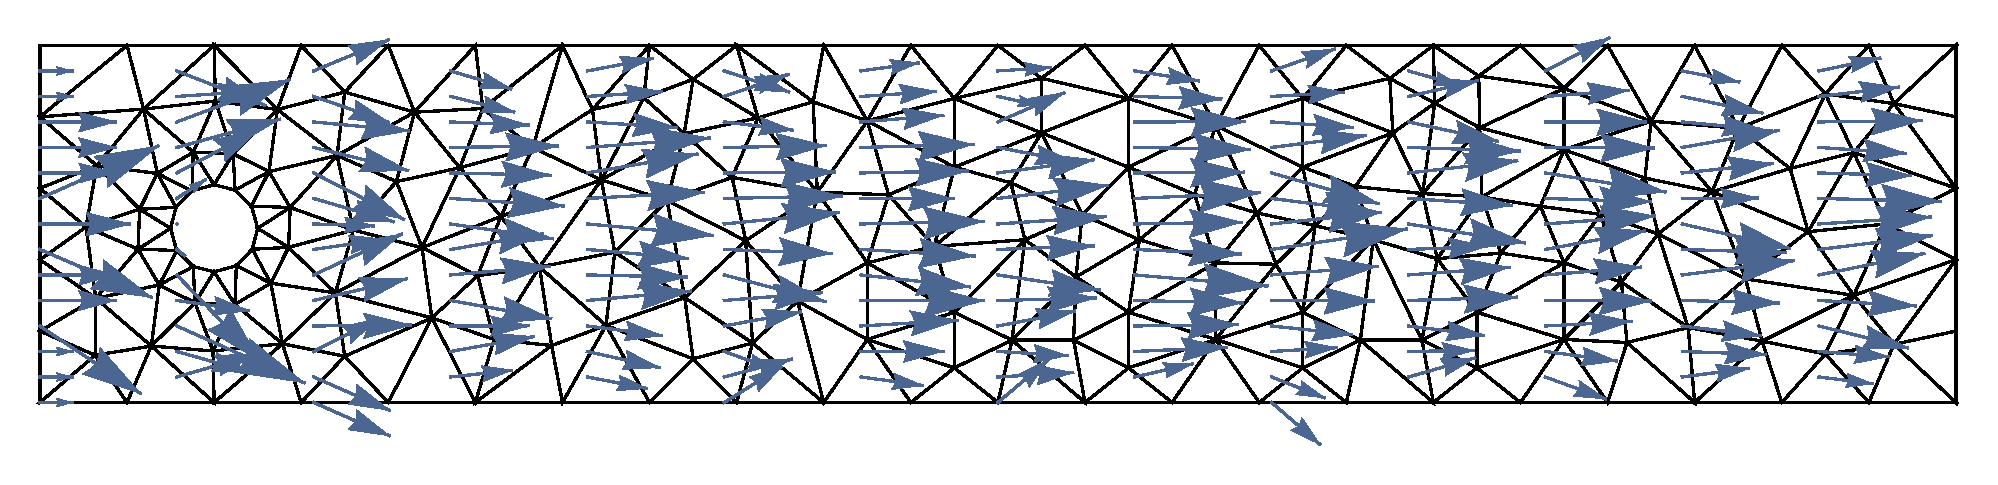
\includegraphics[width=\textwidth]{Figures/01_introduction/P1P0_100.pdf}
\caption{Решение за ламинарен поток чрез (\ref{eq:2D_DFG_Direct_Crank-Nicholson}) след 100 стъпки по времето, с размер на стъпката $\Delta t = 0.01$ }\label{fig:p0p1-plot}
\end{figure}

\begin{figure}[H]
\centering
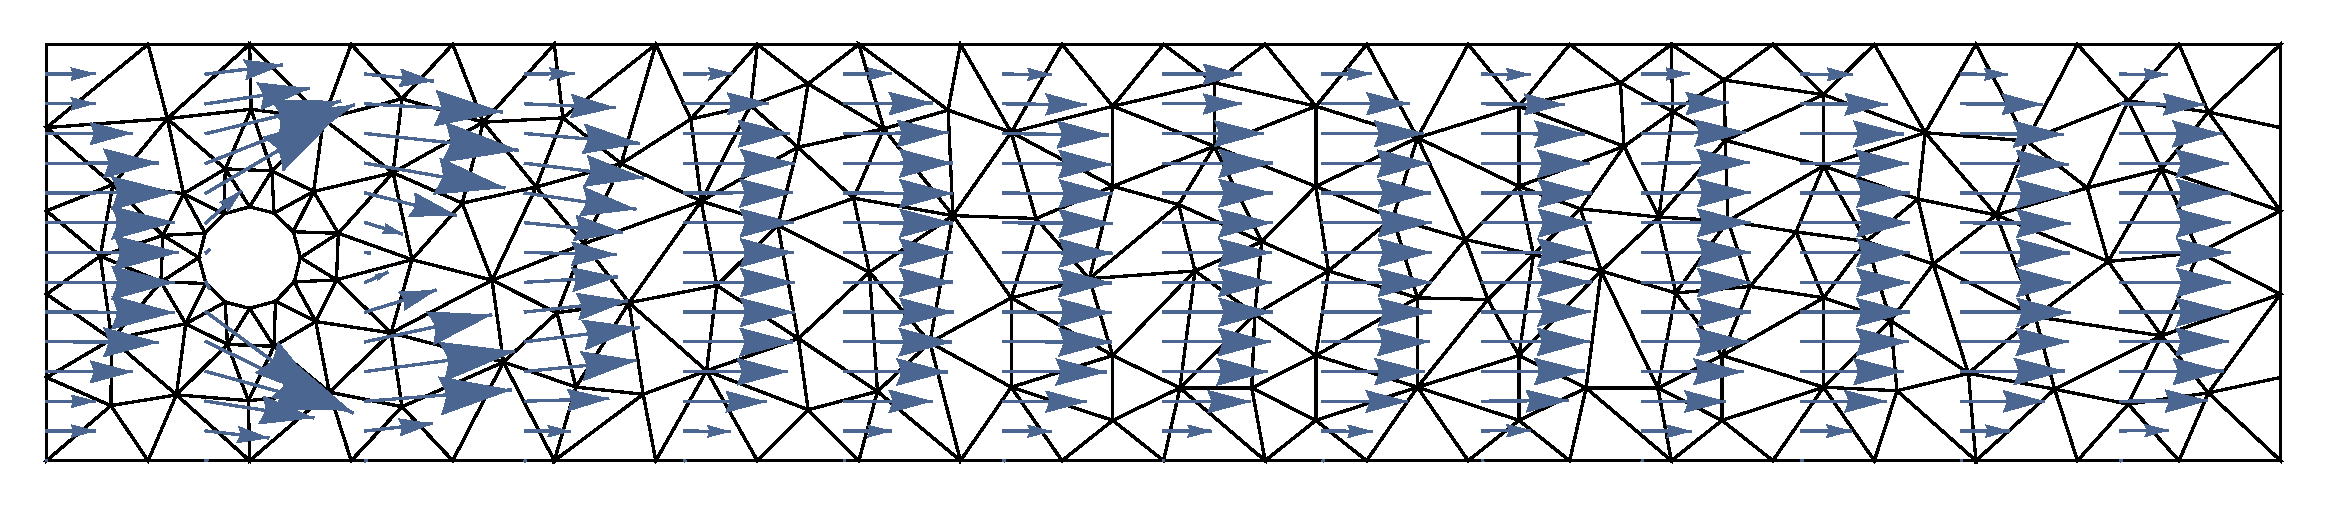
\includegraphics[width=\textwidth]{Figures/01_introduction/P2P1_100.pdf}
\caption{Решение за ламинарен поток чрез (\ref{eq:chorin_split_fem}) след 100 стъпки по времето, с размер на стъпката $\Delta t = 0.01$ }\label{fig:chorin-plot}
\end{figure}

\begin{figure}[H]
\centering
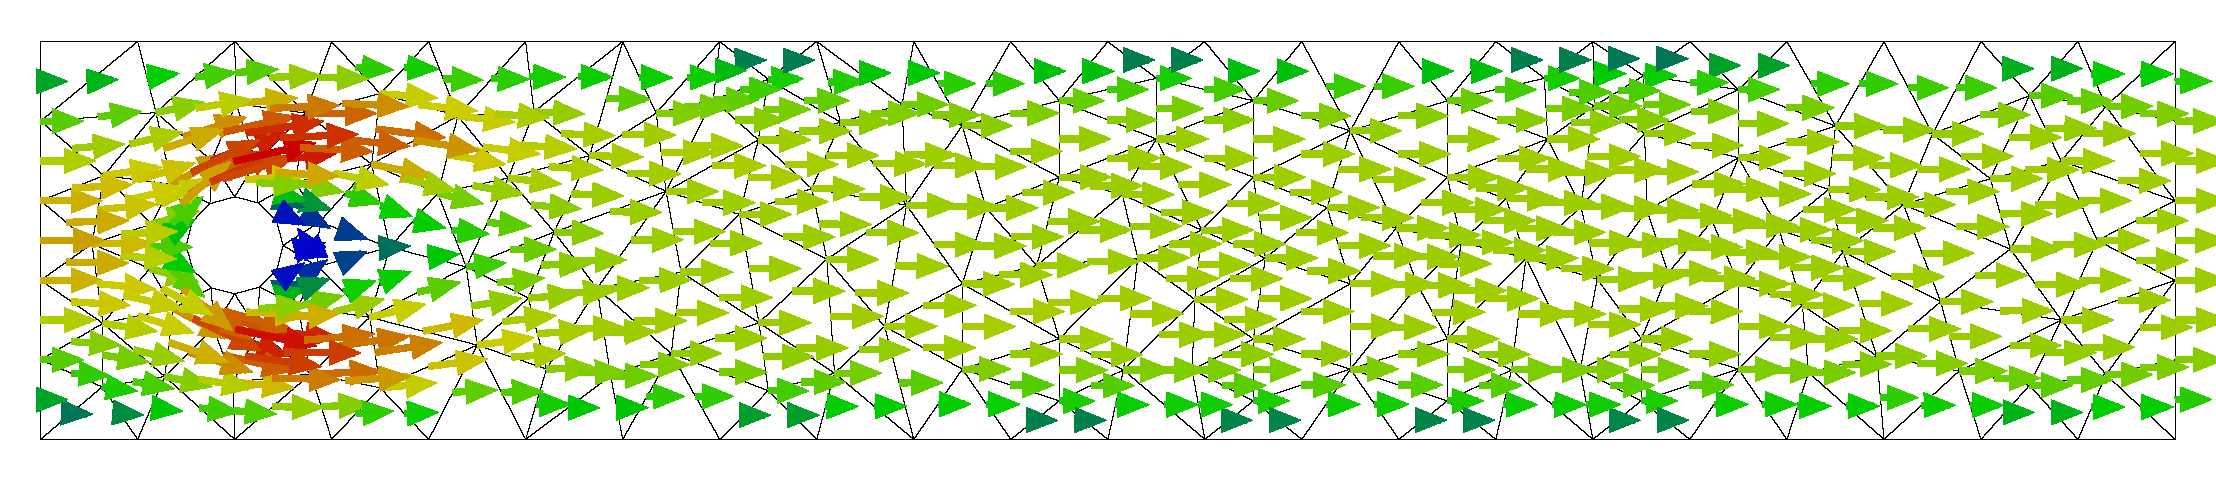
\includegraphics[width=\textwidth]{Figures/01_introduction/P2P1_adv_diff_100.pdf}
\caption{Решение за ламинарен поток чрез (\ref{eq:adv-diff-split-advect})-(\ref{eq:adv-diff-split-velicity-mass}) след 100 стъпки по времето, с размер на стъпката $\Delta t = 0.01$} \label{fig:advection-diffusion-plot}
\end{figure}

\chapter{Паралелна имплементация}\label{ch:FEM-Parallel}
В тази секция ще представим техниките, използвани за многонишкова CPU и GPU имплементация на МКЕ. Ще представим графики, които показват как алгоритмите скалират с увеличаване на броя на (логическите) CPU ядра и как се представят при изпълнение на GPU. Тестовете са извършени върху две машини със следните характеристики: Компютър 1: CPU - Intel(R) Core(TM) i7-3632QM CPU @ 2.20GHz (4 ядра, 8 нишки (логически ядра)), 2 плочки 4GB SODIMM DDR3 Synchronous 800 MHz RAM and Компютър 2: CPU - Intel(R) Core(TM) i7-9700 CPU @ 3.00GHz (8 ядра, 8 нишки (логически ядра)), 4 плочки 16GB DDR4 1333 MHz RAM, GPU - NVidia A5000.

За целта е използвана триангулация със следните размери (вж. Фиг. \ref{tab:mesh_size}).
\begin{figure}[H]
\centering
\begin{tabular}{|c|r|r|}
\hline
Брой елементи               & 305854                      \\ \hline
Брой възли за скоростта        & 613458                      \\ \hline
Брой възли за налягането         & 153802                      \\ \hline
\end{tabular}\caption{Размер на триангулацията, използвана в числените експерименти.}\label{tab:mesh_size}
\end{figure}

Първо, представяме резултатите от еднонишковата имплементация на алгоритъма. Тя ще послужи за основа при последващи сравнения.

\begin{table}[H]
\centering
\begin{tabular}{|c|c|c|c|c|c|c|c|}
\hline
\multirow{3}{*}{} & \multicolumn{7}{c|}{Компютър 1}                                                                                                                                       
\\ \cline{2-8}
& Step 1 & (\ref{eq:adv-diff-split-diffuse}) & (\ref{eq:adv-diff-split-pressure}) & (\ref{eq:adv-diff-split-velicity-mass}) & \begin{tabular}[c]{@{}c@{}}СГ \\ (Общо)\end{tabular} & \begin{tabular}[c]{@{}c@{}}Асемблиране\end{tabular} & \begin{tabular}[c]{@{}c@{}}Общо\\време\end{tabular} \\ \hline
\begin{tabular}[c]{{@{{}}c@{{}}}}Средно\\време\end{tabular}  & 79.75s & 138.33s & 505.50s & 44.47s & 688.30s & 20.80s & 794.82s\\ \hline 
\begin{tabular}[c]{@{}c@{}}Стандартно\\отклонение\end{tabular} & 0.64s&3.83s&3.62s&1.30s&8.76s&0.38s&10.01s\\ \hline
Медиана & 80.20s&141.05s&508.06s&45.39s&694.50s&21.07s&801.89s\\ \hline
Мин. & 79.30s&135.62s&502.94s&43.55s&682.11s&20.54s&787.74s\\ \hline
Макс. & 80.20s&141.05s&508.06s&45.39s&694.50s&21.07s&801.89s\\ \hline
\end{tabular}\caption{Статистика за еднонишково решаване на (\ref{eq:adv-diff-split-advect})-(\ref{eq:adv-diff-split-velicity-mass}) на Компютър 1 за ламинарен поток със стъпка $\Delta t = 0.01$}
\label{tab:computer1-laminar-baseline}
\end{table}

\begin{table}[H]
\centering
\begin{tabular}{|c|c|c|c|c|c|c|c|}
\hline
\multirow{3}{*}{} & \multicolumn{7}{c|}{Компютър 2}                                                                                                                                       
\\ \cline{2-8}
& (\ref{eq:adv-diff-split-advect}) & (\ref{eq:adv-diff-split-diffuse}) & (\ref{eq:adv-diff-split-pressure}) & (\ref{eq:adv-diff-split-velicity-mass}) & \begin{tabular}[c]{@{}c@{}}СГ \\ (Общо)\end{tabular} & \begin{tabular}[c]{@{}c@{}}Асемблиране\end{tabular} & \begin{tabular}[c]{@{}c@{}}Общо\\време\end{tabular} \\ \hline
\begin{tabular}[c]{{@{{}}c@{{}}}}Средно\\време\end{tabular}  & 60.32s & 101.12s & 398.50s & 30.31s & 529.93s & 11.82s & 605.48s\\ \hline 
\begin{tabular}[c]{@{}c@{}}Стандартно\\отклонение\end{tabular} & 0.15s&0.57s&1.85s&0.05s&2.14s&0.04s&2.27s\\ \hline 
Медиана & 60.31s&100.96s&398.29s&30.33s&529.86s&11.84s&605.45s\\ \hline 
Мин. & 60.03s&100.56s&395.98s&30.19s&526.75s&11.76s&602.09s\\ \hline 
Макс & 60.54s&102.54s&402.81s&30.37s&534.01s&11.87s&609.62s\\ \hline
\end{tabular}\caption{Статистика за еднонишково решаване на (\ref{eq:adv-diff-split-advect})-(\ref{eq:adv-diff-split-velicity-mass}) на Компютър 2 за ламинарен поток със стъпка $\Delta t = 0.01$.}
\label{tab:computer2-laminar-baseline}
\end{table}

%%%%%%%%%%%%%%%%%%%%%%%%%%%%%%%%%%%%%%%%%%%%%%%%%%%%%%%%%%%%%%%%%%%%%%%%%%
%%%%%%%%%%%%%%%%%%%%%%%%%%% TURBULENT %%%%%%%%%%%%%%%%%%%%%%%%%%%%%%%%%%%%
%%%%%%%%%%%%%%%%%%%%%%%%%%%%%%%%%%%%%%%%%%%%%%%%%%%%%%%%%%%%%%%%%%%%%%%%%%

\begin{table}[H]
\centering
\begin{tabular}{|c|c|c|c|c|c|c|c|}
\hline
\multirow{3}{*}{} & \multicolumn{7}{c|}{Компютър 1}                                                                                                                                       
\\ \cline{2-8}
& (\ref{eq:adv-diff-split-advect}) & (\ref{eq:adv-diff-split-diffuse}) & (\ref{eq:adv-diff-split-pressure}) & (\ref{eq:adv-diff-split-velicity-mass}) & \begin{tabular}[c]{@{}c@{}}СГ \\ (Общо)\end{tabular} & Асемблиране & \begin{tabular}[c]{@{}c@{}}Общо\\време\end{tabular} \\ \hline
\begin{tabular}[c]{{@{{}}c@{{}}}}Средно\\време\end{tabular}  & 80.35s & 196.81s & 597.43s & 55.31s & 849.54s & 20.45s & 956.29s\\ \hline 
\begin{tabular}[c]{@{}c@{}}Стандартно\\отклонение\end{tabular} & 0.83s&5.57s&3.18s&0.77s&9.52s&0.08s&10.45s\\ \hline
Медиана & 80.94s&200.74s&599.68s&55.86s&856.28s&20.51s&963.68s\\ \hline
Мин. & 79.76s&192.87s&595.18s&54.76s&842.81s&20.40s&948.90s\\ \hline
Макс. & 80.94s&200.74s&599.68s&55.86s&856.28s&20.51s&963.68s\\ \hline
\end{tabular}\caption{Статистика за еднонишково решаване на (\ref{eq:adv-diff-split-advect})-(\ref{eq:adv-diff-split-velicity-mass}) на Компютър 1 за турбулентен поток със стъпка $\Delta t = 0.01$}
\label{tab:computer1-turbulent-baseline}
\end{table}

\begin{table}[H]
\centering
\begin{tabular}{|c|c|c|c|c|c|c|c|}
\hline
\multirow{3}{*}{} & \multicolumn{7}{c|}{Компютър 2}                                                                                                                                       
\\ \cline{2-8}
& (\ref{eq:adv-diff-split-advect}) & (\ref{eq:adv-diff-split-diffuse}) & (\ref{eq:adv-diff-split-pressure}) & (\ref{eq:adv-diff-split-velicity-mass}) & \begin{tabular}[c]{@{}c@{}}СГ \\ (Общо)\end{tabular} & Асемблиране & \begin{tabular}[c]{@{}c@{}}Общо\\Време\end{tabular} \\ \hline
\begin{tabular}[c]{{@{{}}c@{{}}}}Средно\\Време\end{tabular}  & 61.22s & 143.49s & 541.06s & 37.69s & 722.23s & 11.90s & 798.78s\\ \hline
\begin{tabular}[c]{@{}c@{}}Стандартно \\ Отклонение\end{tabular} & 0.31s&0.77s&3.23s&0.17s&3.97s&0.12s&4.25s\\ \hline
Медиана & 61.35s&143.62s&542.91s&37.73s&724.74s&11.89s&801.48s\\ \hline
Мин. & 60.74s&142.42s&535.43s&37.39s&716.07s&11.75s&792.43s\\ \hline
Макс. & 61.71s&144.89s&544.70s&38.03s&727.36s&12.17s&804.32s\\ \hline
\end{tabular}\caption{Статистика за еднонишково решаване на (\ref{eq:adv-diff-split-advect})-(\ref{eq:adv-diff-split-velicity-mass}) на Компютър 2 за турбулентен поток със стъпка $\Delta t = 0.01$.}
\label{tab:computer2-turbulent-baseline}
\end{table}

\section{Асемблиране на глобалните матрици}
В постановката, която разглеждаме, геометрията и матриците не се изменят във времето. По тази причина е достатъчно да асемблираме матриците веднъж. За целта всяка матрица се асемблира на отделна нишка, паралелно с останалите. Тъй като има 5 матрици са нужни 5 нишки. Времето за асемблиране е приблизително равно на времето за асемблиране на най-времеемката матрица.

\section{Многонишкова имплементация на адвекцията}
Тъй като пресмятането на скоростта в момент $t + \Delta t$ не зависи от скоростта в другите възли в момент $t + \Delta t$, паралелната имплементация е тривиална (както зa CPU, така и за GPU). Разделяме възлите от триангулацията на $n$ равни части, където $n$ е броят на (логическите) ядра, с които разполагаме. Всяко ядро пресмята скоростта на всички възли в съответното множество от възли. В частност, ако искаме да пресметнем $m$ стойности и разполагаме с $m$ ядра, всяко от тях може да пресметне една стойност независимо от останалите.

Основните заявки, които трябва да можем да изпълняваме при имплементация на полу-Лагранжевия метод са: намиране на елемент, съдържащ конкретна точка, и намиране на възел от триангулацията, който се намира най-близо до дадена точка в пространството. Двете операции могат да бъдат имплементирани ефективно с помощта на KD дърво, което е подробно разгледано в дипломната работа. KD дърветата намират широко разпространение в компютърната графика при ray-tracing алгоритмите \cite{pbrt}. С малка модификация на алгоритъма за пресичане на лъч можем да получим ефективна имплементация на заявката за намиране на елемент съдържащ дадена точка. Намирането на точка от дадено множество точки, която е най-близко до друга точка в пространството, е класическа задача в сферата на изкуствения интелект, представена в \cite{knn-ai}. Изключително важно за големи триангулации е да получим балансирано дърво.

\begin{figure}[H]
  \centering
  \begin{subfigure}[b]{0.49\textwidth}
      \centering
      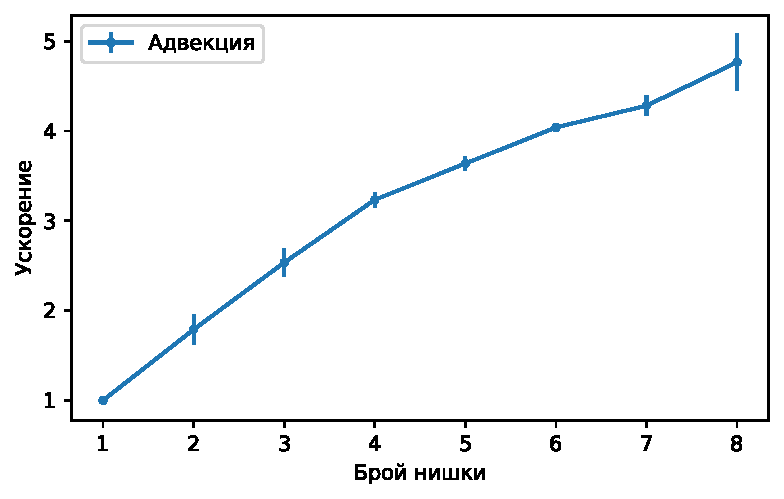
\includegraphics[width=\textwidth]{Figures/BG/LaminarAdvectionSpeedUpC1.pdf}
      \caption{Компютър 1}
  \end{subfigure}
  \begin{subfigure}[b]{0.49\textwidth}
      \centering
      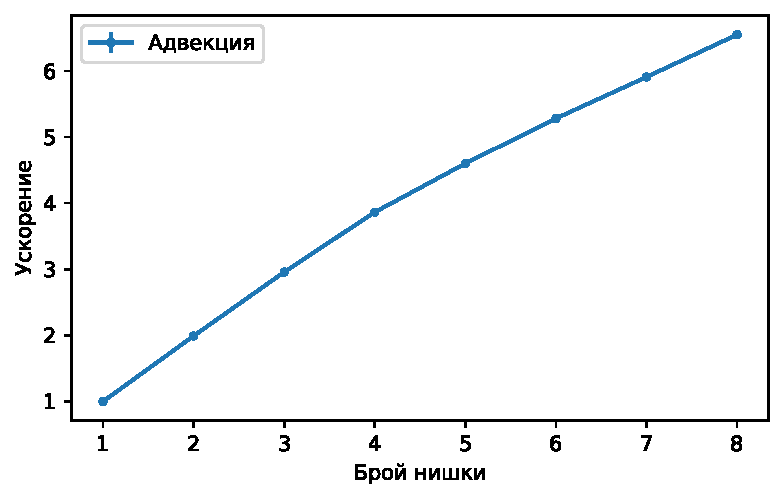
\includegraphics[width=\textwidth]{Figures/BG/LaminarAdvectionSpeedUpC2.pdf}
      \caption{Компютър 2}
  \end{subfigure}
\caption{Скалиране на производителността на полу-Лагранжевия метод за ламинарен поток. Вертикалните линии са с големина 2 пъти стандартното отклонение.}\label{fig:advection_speedup_graph_laminar}
\end{figure}

\begin{figure}[H]
  \centering
  \begin{subfigure}[b]{0.49\textwidth}
      \centering
      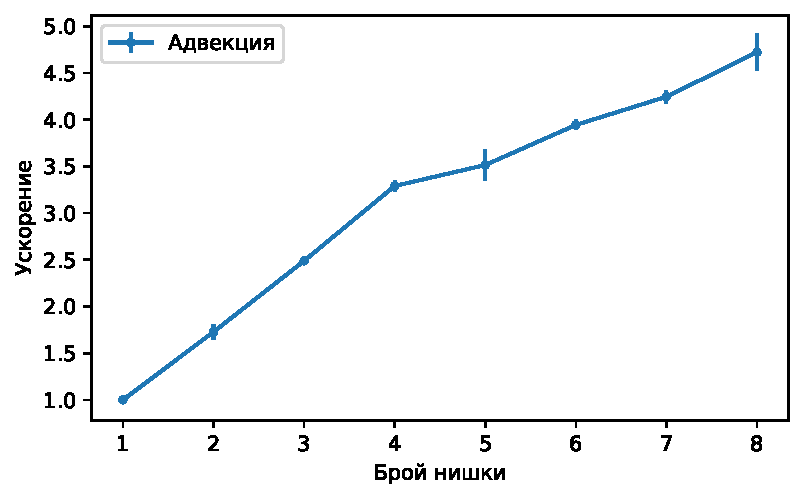
\includegraphics[width=\textwidth]{Figures/BG/TurbulentAdvectionSpeedUpC1.pdf}
      \caption{Комоютър 1}
  \end{subfigure}
  \begin{subfigure}[b]{0.49\textwidth}
      \centering
      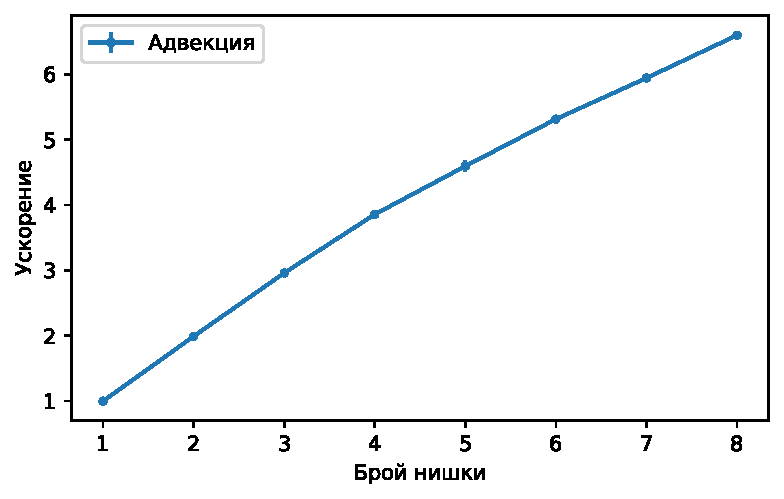
\includegraphics[width=\textwidth]{Figures/BG/TurbulentAdvectionSpeedUpC2.pdf}
      \caption{Компютър 2}
  \end{subfigure}
\caption{Скалиране на производителността на полу-Лагранжевия метод за турбулентен поток. Вертикалните линии са с големина 2 пъти стандартното отклонение.}\label{fig:advection_speedup_graph_turbulent}
\end{figure}

\section{Метод на спрегнатия градиент}
За разлика от полу-Лагранжевия метод, методът на спрегнатия градиент не може да бъде директно имплементиран в многонишкова среда, без използването на сихнронизационни примитиви. Причината за това са двете скаларни произведения в него. Те играят ролята на ``бариера'', т.е. всички нишки трябва да спрат и да изчакат пресмятането на скаларното произведение да завърши преди да продължат със следващата стъпка. Въпреки това, отделните стъпки на алгоритъма могат да бъдат имплементирани в паралелна среда (повече подробности за това са представени в дипломната работа). Представяме графики, показващи как се скалира производителността на метода с увеличаване на броя на (логическите) ядра.

\begin{figure}[H]
  \centering
  \begin{subfigure}[b]{0.8\textwidth}
      \centering
      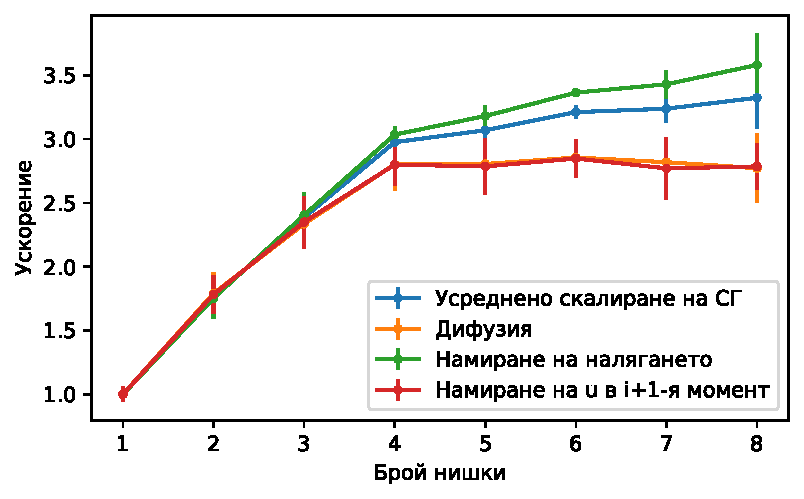
\includegraphics[width=\textwidth]{Figures/BG/LaminarCGSpeedUpC1.pdf}
      \caption{Компютър 1}
  \end{subfigure}
\end{figure}
\begin{figure}[H]
	\centering
  \ContinuedFloat
  \begin{subfigure}[b]{0.8\textwidth}
      \centering
      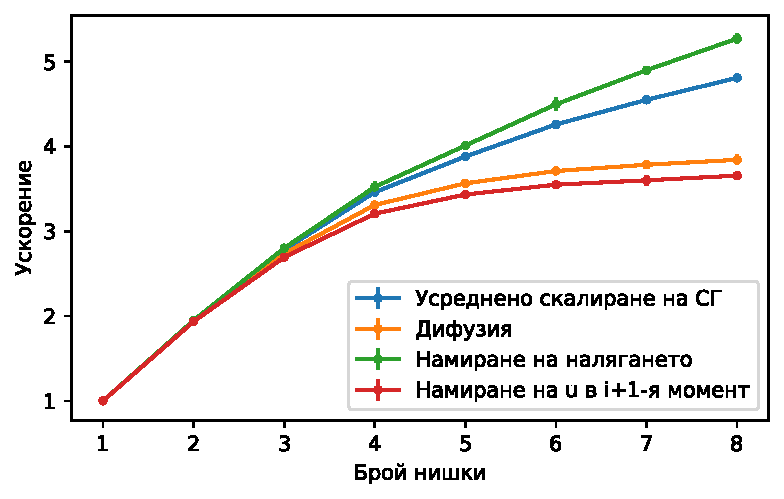
\includegraphics[width=\textwidth]{Figures/BG/LaminarCGSpeedUpC2.pdf}
      \caption{Компютър 2}
  \end{subfigure}\caption{Скалиране на метода на спрегнатия градиент за ламинарен поток. Вертикалните линии са с големина 2 пъти стандартното отклонение.}
  \label{fig:laminar-scaling}
\end{figure}


%%%%%%%%%%%%%%%%%%%%%%%%%%%%%%%%%%%%%%%%%%%%%%%%%%%%%%%
%%%%%%%%%%%%%%%%%%%%%% TURBULENT %%%%%%%%%%%%%%%%%%%%%%
%%%%%%%%%%%%%%%%%%%%%%%%%%%%%%%%%%%%%%%%%%%%%%%%%%%%%%%
\begin{figure}[H]
  \centering
  \begin{subfigure}[b]{0.8\textwidth}
      \centering
      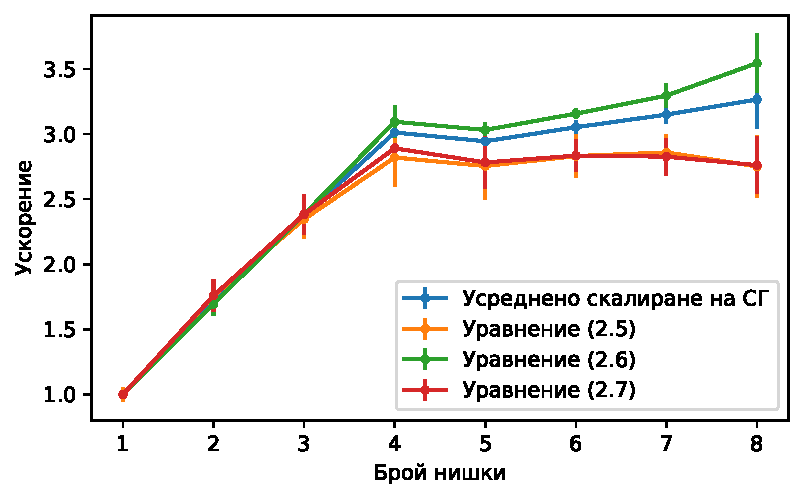
\includegraphics[width=\textwidth]{Figures/BG/TurbulentCGSpeedUpC1.pdf}
      \caption{Компютър 1}
  \end{subfigure}
\end{figure}
\begin{figure}[H]
	\centering
  \ContinuedFloat
  \begin{subfigure}[b]{0.8\textwidth}
      \centering
      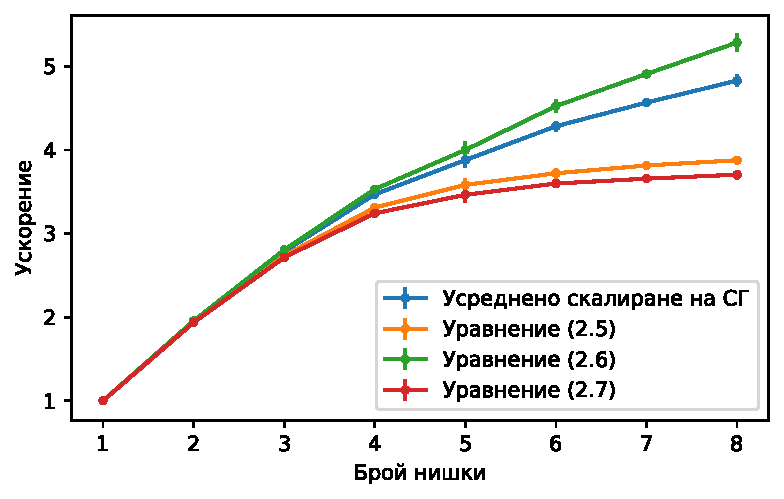
\includegraphics[width=\textwidth]{Figures/BG/TurbulentCGSpeedUpC2.pdf}
      \caption{Компютър 2}
  \end{subfigure}\caption{Скалиране на метода на спрегнатия градиент за турбулентен поток. Вертикалните линии са с големина 2 пъти стандартното отклонение.}
  \label{fig:turbulent-scaling}
\end{figure}

От графиките можем да видим че производителността се скалира по-зле при добавяне на (логически) ядра, в сравнение с полу-Лагранжевия метод. Причината е, че отделните стъпки от алгоритъма са твърде прости, и не могат да ``заситят'' процесора. За да се скалира задачата, трябва матрицата, участваща в метода, да бъде голяма, както и методът да има нужда от голям брой итерации.

\subsection{Преобуславяне}
Имайки предвид, че по-голямата част от времето за решаване на задачата се прекарва в метода на спрегнатия градиент, преобуславяне чрез IC0 е имплементирано с цел да се подобри производителността. Паралелното изчисляване и паралелното прилагане на преобусловителя са трудни задачаи, които ще бъдат обект на следващо проучване. По тази причина те са имплементирани на една нишка. Представяме резултати от изпълнението
\begin{table}[H]
\centering
\begin{tabular}{|c|c|c|c|}
\hline Задача
& \begin{tabular}[c]{@{}c@{}}Брой итерации\\ (\ref{eq:adv-diff-split-diffuse})\end{tabular} & \begin{tabular}[c]{@{}c@{}}Брой итерации\\ (\ref{eq:adv-diff-split-pressure})\end{tabular} & \begin{tabular}[c]{@{}c@{}}Брой итерации\\ (\ref{eq:adv-diff-split-velicity-mass})\end{tabular} \\ \hline
Ламинарен поток         & 10370& 195422 &    2763 \\ \hline
Турбулентен поток       & 14820& 264394 &   3504 \\ \hline
Ламинарен поток (IC0)   &  1855&  72353 &    495\\ \hline
Турбулентен поток (IC0) &  2693&  85047 &    693\\ \hline
\end{tabular}\caption{Общ брой итерации за всяка една система.}\label{tab:CG-iterations}
\end{table}

% ====================================================================================================
% =========================================== COMPUTE IC0 ============================================
% ====================================================================================================

\begin{table}[H]
\centering
\begin{tabular}{|c|c|c|c|c|c|}
\hline
                                                                                   & \begin{tabular}[c]{@{}c@{}}Средно\\ време\end{tabular} & Медиана & SD   & \begin{tabular}[c]{@{}c@{}}Мин.\\ време\end{tabular} & \begin{tabular}[c]{@{}c@{}}Макс.\\ време\end{tabular} \\ \hline
\begin{tabular}[c]{@{}c@{}}Пресмятане на IC0 за\\ Матрица на коравината на налягането\end{tabular} & 15.66                                               & 15.67  & 0.02 & 15.64                                              & 15.68                                              \\ \hline
\begin{tabular}[c]{@{}c@{}}Пресмятане IC0 за\\ Матрица на маста за скоростта\end{tabular}      & 390.33                                              & 389.98 & 1.32 & 389.22                                             & 391.79                                             \\ \hline
\begin{tabular}[c]{@{}c@{}}Пресмятане IC0 за\\ Дифузионна матрица\end{tabular}          & 380.68                                              & 379.17 & 4.98 & 376.62                                             & 386.23                                             \\ \hline
\end{tabular}\caption{Времето нужно за пресмятане на всяка една преобуславяща матрица на Компютър 2}\label{tab:ic0-timings}
\end{table}

\begin{table}[H]
\centering
\begin{tabular}{|c|c|c|c|c|c|}
\hline
     & \begin{tabular}[c]{@{}c@{}}Средно\\ Време\end{tabular} & Медиана & \begin{tabular}[c]{@{}c@{}}Стандартно \\ Отклонение\end{tabular}   & \begin{tabular}[c]{@{}c@{}}Минимално\\ Време\end{tabular} & \begin{tabular}[c]{@{}c@{}}Максимално\\ Време\end{tabular} \\ \hline
(\ref{eq:adv-diff-split-diffuse}) & 54.76 & 54.76  & 0.00 & 74.75 & 54.76 \\ \hline
(\ref{eq:adv-diff-split-pressure}) & 393.30 & 393.50 & 0.29 & 393.09 & 393.50  \\ \hline
(\ref{eq:adv-diff-split-velicity-mass}) & 22.01 & 22.03  & 0.03 & 21.99 & 22.03  \\ \hline
\end{tabular}\caption{Време за решаване на (\ref{eq:adv-diff-split-diffuse})-(\ref{eq:adv-diff-split-velicity-mass}) с преобуславяне на една нишка на Компютър 2.}\label{tab:solve-ic0-1-thread}
\end{table}

От резултатите можем да видим, че, въпреки че броят на итерациите е сериозно намален, времето за изпълнение е не е много по-добро (дори сравнено с еднонишковата имплементация без преобуславяне). Резултатите обаче показват потенциал за подобрения на цялостното бързодействие, ако преобуславянето бъде ефективно разпаралелено.

\section{GPU имплементация}
\subsection{Кратко въведение в програмия модел}
Тук ще опишем графичните процесори, произвеждани от NVidia. На практика, обаче, архитектурата на графичните процесори не варира драстично при различните производители. Централните процесори (CPU) са изключително сложни. Те имат малко на брой ядра, в сравнение с графичните процесори. За да подобрят скоростта си, централните процесори имат много различни системи (служещи за branch prediction, prefetching, cache, out-of-order execution, pipelining и т.н.). От друга страна, ядрата на графичните процесори са изключително прости, но за сметка на това са много на брой. В един графичен процесор има няколко на брой Streaming Multiprocessor-а (SM). Всеки от тях е отговорен за извличане на данни и операции от паметта на графичния процесор, както и за разпределяне на работата между нишките. Всяка инструкция се изпълнява \textit{едновременно} от 32 нишки (warp) върху различни данни. Ако се стигне до условен оператор, при който част от нишките трябва да изпълнят един клон, а другите друг, двата клона се изпълняват, като в зависимост от това кой клон се изпълнява, част от нишките са неактивни. На всеки процесорен цикъл SM избира warp от активни нишки (такива, които не чакат да пристигнат данни от паметта или някоя операция да завърши) и изпълнява една или повече операции с него.  
\subsection{Асемблиране на глобалните матрици}
Както беше споменато, при разредените матрични формати се създават зависимостти между данните, поради което тези алгоритми не пасват добре на GPU програмния модел. GPU имплементацията на асемблирането е оставена за бъдещо проучване. За нашите цели ще асемблираме матриците на CPU, с алгоритъма, който представихме.
\subsection{Адвекция}
За имплементацията на полу-Лагранжевия метод може да бъде използван същият подход като при CPU имплементацията. В този случай всяка GPU нишка отговаря за пресмятането на скоростта в един възел от триангулацията. От изключителна важност при имплементацията на KD дървото за GPU е обхождането му да не бъде имплементирано чрез рекурсия, а чрез стек и цикъл, симулиращи рекурсия. 
\subsection{Метод на спрегнатия градиент}
Както вече беше споменато, двете скаларни произведения действат като бариери, което пречи за директна паралелна имплементация. Разглеждаме два подхода: при първия (multi kernel) всяка стъпка от алгоритъма е имплементирана като отделна GPU функция (kernel). При втория подход (mega kernel), целият алгоритъм се изпълнява на GPU, но се налага използването на глобална синхронизационна примитива. По-старите графични процесори и езици за програмиране не разполагат с вградени такива примитиви.
\subsection{Резултати}

\begin{table}[H]
\centering
\begin{tabular}{|c|c|c|c|c|c|c|c|}
\hline
\multirow{3}{*}{} & \multicolumn{7}{c|}{GPU Multi Kernel подход}                                                                                                                                       
\\ \cline{2-8}
& (\ref{eq:adv-diff-split-advect}) & (\ref{eq:adv-diff-split-diffuse}) & (\ref{eq:adv-diff-split-pressure}) & (\ref{eq:adv-diff-split-velicity-mass}) & \begin{tabular}[c]{@{}c@{}}СГ \\ (Общо)\end{tabular} & Асемблиране & \begin{tabular}[c]{@{}c@{}}Общо\\време\end{tabular} \\ \hline
\begin{tabular}[c]{{@{{}}c@{{}}}}Средно\\време\end{tabular}  & 0.56s & 14.67s & 65.96s & 4.71s & 85.34s & 4.02s & 91.16s\\ \hline
\begin{tabular}[c]{@{}c@{}}Стандартно\\отклонение\end{tabular} & 0.01s&0.07s&0.34s&0.02s&0.35s&0.02s&0.36s\\ \hline
Медиана & 0.56s&14.69s&66.00s&4.71s&85.35s&4.02s&91.19s\\ \hline
Мин. & 0.53s&14.56s&65.33s&4.69s&84.81s&3.99s&90.62s\\ \hline
Макс. & 0.57s&14.75s&66.47s&4.74s&85.87s&4.03s&91.69s\\ \hline
\end{tabular}\caption{Време за решаване на (\ref{eq:adv-diff-split-advect})-(\ref{eq:adv-diff-split-velicity-mass}), чрез графичен процесор, за ламинарен поток със стъпка $\Delta t = 0.01$. Използван е multi kernel подходът.}
\end{table}

\begin{table}[H]
\centering
\begin{tabular}{|c|c|c|c|c|c|c|c|}
\hline
\multirow{3}{*}{} & \multicolumn{7}{c|}{GPU Multi Kernel подход}                                                                                                                                       
\\ \cline{2-8}
& (\ref{eq:adv-diff-split-advect}) & (\ref{eq:adv-diff-split-diffuse}) & (\ref{eq:adv-diff-split-pressure}) & (\ref{eq:adv-diff-split-velicity-mass}) & \begin{tabular}[c]{@{}c@{}}СГ \\ (Общо)\end{tabular} & Асемблиране & \begin{tabular}[c]{@{}c@{}}Общо\\време\end{tabular} \\ \hline
\begin{tabular}[c]{{@{{}}c@{{}}}}Средно\\време\end{tabular}  & 0.84s & 20.69s & 78.12s & 5.70s & 104.50s & 4.03s & 110.63s\\ \hline
\begin{tabular}[c]{@{}c@{}}Стандартно\\отклонение\end{tabular} & 0.01s&0.04s&0.25s&0.01s&0.25s&0.02s&0.23s\\ \hline
Медиана & 0.85s&20.71s&78.12s&5.70s&104.56s&4.02s&110.66s\\ \hline
Мин. & 0.83s&20.61s&77.75s&5.69s&104.15s&4.01s&110.33s\\ \hline
Макс. & 0.86s&20.73s&78.55s&5.72s&104.99s&4.07s&111.11s\\ \hline
\end{tabular}\caption{Време за решаване на (\ref{eq:adv-diff-split-advect})-(\ref{eq:adv-diff-split-velicity-mass}), чрез графичен процесор, за турбулентен поток със стъпка $\Delta t = 0.01$. Използван е multi kernel подходът.}
\end{table}

%%%%%%%%%%%%%%%%%%%%%%%%%%%%%%%%%%%%%%%%%%%%%%%%%%%%%%%%%%%%%%%
%%%%%%%%%%%%%%%%%%%%%%%%% MEGAKERNEL %%%%%%%%%%%%%%%%%%%%%%%%%%
%%%%%%%%%%%%%%%%%%%%%%%%%%%%%%%%%%%%%%%%%%%%%%%%%%%%%%%%%%%%%%%

\begin{table}[H]
\centering
\begin{tabular}{|c|c|c|c|c|c|c|c|}
\hline
\multirow{3}{*}{} & \multicolumn{7}{c|}{GPU Mega Kernel подход}                                                                                                                                       
\\ \cline{2-8}
& (\ref{eq:adv-diff-split-advect}) & (\ref{eq:adv-diff-split-diffuse}) & (\ref{eq:adv-diff-split-pressure}) & (\ref{eq:adv-diff-split-velicity-mass}) & \begin{tabular}[c]{@{}c@{}}СГ\\(Общо)\end{tabular} & Асемблиране & \begin{tabular}[c]{@{}c@{}}Общо\\време\end{tabular} \\ \hline
\begin{tabular}[c]{{@{{}}c@{{}}}}Средно\\време\end{tabular}  & 0.54s & 2.98s & 8.19s & 1.26s & 12.44s & 4.02s & 18.24s\\ \hline
\begin{tabular}[c]{@{}c@{}}Стандартно\\отклонение\end{tabular} & 0.01s&0.07s&0.09s&0.01s&0.06s&0.02s&0.06s\\ \hline
Медиана & 0.54s&2.96s&8.20s&1.26s&12.43s&4.02s&18.22s\\ \hline
Мин. & 0.53s&2.95s&7.95s&1.25s&12.36s&3.99s&18.13s\\ \hline
Макс. & 0.55s&3.18s&8.29s&1.28s&12.54s&4.05s&18.32s\\ \hline
\end{tabular}\caption{Време за решаване на (\ref{eq:adv-diff-split-advect})-(\ref{eq:adv-diff-split-velicity-mass}), чрез графичен процесор, за ламинарен поток със стъпка $\Delta t = 0.01$. Използван е mega kernel подходът.}
\end{table}

\begin{table}[H]
\centering
\begin{tabular}{|c|c|c|c|c|c|c|c|}
\hline
\multirow{3}{*}{} & \multicolumn{7}{c|}{GPU Mega Kernel подход}                                                                                                                                       
\\ \cline{2-8}
& (\ref{eq:adv-diff-split-advect}) & (\ref{eq:adv-diff-split-diffuse}) & (\ref{eq:adv-diff-split-pressure}) & (\ref{eq:adv-diff-split-velicity-mass}) & \begin{tabular}[c]{@{}c@{}}СГ \\ (Общо)\end{tabular} & Асемблиране & \begin{tabular}[c]{@{}c@{}}Общо\\време\end{tabular} \\ \hline
\begin{tabular}[c]{{@{{}}c@{{}}}}Средно\\време\end{tabular}  & 0.84s & 4.01s & 9.72s & 1.45s & 15.18s & 4.00s & 21.26s\\ \hline
\begin{tabular}[c]{@{}c@{}}Стандартно\\отклонение\end{tabular} & 0.00s&0.01s&0.04s&0.00s&0.04s&0.01s&0.05s\\ \hline
Медиана & 0.84s&4.01s&9.70s&1.45s&15.17s&4.00s&21.27s\\ \hline
Мин. & 0.83s&3.99s&9.67s&1.44s&15.12s&3.98s&21.20s\\ \hline
Макс. & 0.84s&4.02s&9.79s&1.46s&15.24s&4.02s&21.32s\\ \hline
\end{tabular}\caption{Време за решаване на (\ref{eq:adv-diff-split-advect})-(\ref{eq:adv-diff-split-velicity-mass}), чрез графичен процесор, за турбулентен поток със стъпка $\Delta t = 0.01$. Използван е mega kernel подходът.}
\end{table}
От резултатите можем да се убедим, че вторият метод (mega kernel) е по-ефективен.

\section{Сравнение}
От резултатите се вижда, че графичният процесор има по-добра производителност. Това в никакъв случай не означава, че ерата на централните процесори е преминала. Трудно е да се сравняват толкова различни по същество хардуерни устройства, тъй като няма еднозначни критерии, по-които това да се направи. Графичният процесор, използван за числените експерименти, е висок клас, докато централните процесори са по-скоро в средния (към нисък) клас централни процесори. Графичните процесори обикновено разполагат с по-малко памет от централните процесори и няма опция за добавяне на допълнително количество памет. Има нужда от повече тестове на различни постановки с различни по големина области. Това, което можем да заключим от този експеримент, е, че има перспектива в имплементацията на МКЕ за графични процесори. Както се вижда, те се справят добре, когато има множество независими прости изчисления. Има обаче множество отворени въпроси:
\begin{itemize}
\item Колко добре биха се справили графичните процесори с дискретизацията на областта?
\item Колко добре биха се справили графичните процесори с асемблирането на глобални матрици?
\item Kолко добре биха се справили графичните процесори с изчислението на преобуславяща матрица?
\item Колко добре биха се справили графичните процесори с прилагането на преобуславяща матрица?
\item Колко добре биха се справили графичните процесори с построяването на KD дървета?
\end{itemize}
Най-вероятно графичните процесори няма да могат да се справят добре с някои от тези задачи и част от тях ще трябва да се имплементират за CPU.

\chapter*{Заключение} 
\addcontentsline{toc}{chapter}{Заключение}
В дипломната работа бяха изложени 3 подхода за решаване на уравненията на Navier-Stokes. Един от тях беше най-подходящ за нашите цели (добра производителност и възможност за ефективна паралелна реализация) и беше имплементиран, както за CPU, така и за GPU. Избраният алгоритъм разделя диференциалния оператор по времето на три части: адвекция, дифузия и уравнение на Поасон относно налягането. Полу-Лагранжевият метод беше приложен за решаване на адвекцията и беше показано, че дава добри резултати както на CPU, така и на GPU. Дифузията и уравнението за налягането се свеждат до решаване на линейна система с положително определена матрица. Методът на спрегнатия градиент беше използван за решаването на тези системи. За GPU имплементацията бяха разработени два подхода: multi kernel и mega kernel и беше показано, че mega kernel подходът е значително по-бърз. Въпреки че реализацията на този подход е лесна, не ни е известно в литературата той да е разглеждан и да са правени сравнения с multi kernel подхода. Метод с преобуславяне с непълна факторизация на Холецки беше имплементиран. Въпреки че преобуславянето намалява значително броя на итерации при метода на спрегнатия градиент, то не подобрява значително времето за изпълнение, тъй като самото прилагане на преобуславящата матрица, увеличава времето нужно за една итерация на метода. Като резултат в дипломната работа е показано, че използването на GPU за решаване на уравненията на Navier--Stokes би имало своите приложения, като са очертани и посоки за бъдещо развитие в тази посока.

\printbibliography
\end{document}
